\subsection{Models B.}
In this second case, given the symmetry of the problem, we have that, at equilibrium the deviatoric component of the stress tensor $\mathbb{T}$ vanishes. Combining this information with the boundary condition and solving the system~(\ref{sys1B})-(\ref{sys2B}) for its equilibrium, we obtain the same equations as for model A, while the pressure is now defined as:
\begin{equation}
p = \frac{\partial \psi_{vol}}{\partial J} .\label{presB}%= \frac{\kappa}{1+C_s v_s}.
\end{equation}

We follow two different approaches, in case $BA$, we derive the constitutive equation for $\psi_{vol}$, so that the model B and model A predict the same equilibrium behaviour, i.e. $p_A=p_{BA}$. Using Equations~(\ref{presA})-(\ref{presB}), and the constraint $\psi_{vol}(1)=0$, we obtain:
\begin{equation}
\frac{\partial \psi^{BA}_{vol}}{\partial J}= G^A_{eq} \frac{J^{2/3}-1}{J} \Longrightarrow \psi_{vol} = \frac{G^{BA}_{vol}}{2}\left[3(J^{2/3} -1) - 2\ln J\right],
\end{equation}
which is equivalent to using a Neo-Hookean model also for the volumetric spring with shear modulus $G^{BA}_{vol}$. In the second case, we instead consider a more commonly used constitutive model for volumetric deformation. Based on Equation~(\ref{psivol}), the pressure is given by:
\begin{equation}
p_{B} = \frac{\kappa}{1+C_s v_s}.
\end{equation}
Consequently, while Equation~(\ref{eqion}) still hold, we have that also the equilibrium condition~(\ref{eqF}) is now of the form:
\begin{equation}
\begin{aligned}
F_{B}(C_s; c_0,\chi,\kappa)=&\frac{1+C_sv_s+\chi}{(1+C_sv_s)^2}+\frac{\kappa v_s}{k_BT} \frac{1}{1+C_sv_s}+\ln \frac{C_sv_s}{1+C_sv_s}\\[1.5mm]
& +2c_0v_s-\sqrt{\left(\frac{z_fC_f}{C_s}\right)^2+4v_s^2c^2_0} =0 \label{eqFb}
\end{aligned}
\end{equation}
\subsection{Comparison of the Models.}

By construction, the model $A$ and $BA$ agrees. On the other hand, as illustrated in Figure~\ref{Exp1}(b), the discrepancy with model B depends on the real elastic properties of the material tested. In particular, the softer the tissue, the larger is the difference between the two. Looking at Figure~\ref{Exp1}(b), the major discrepancy is in the equilibrium behaviour at the two limits: $c_0$ small and $c_0$ large. 

\begin{figure}[h]
	\begin{subfigure}{0.6\textwidth}
		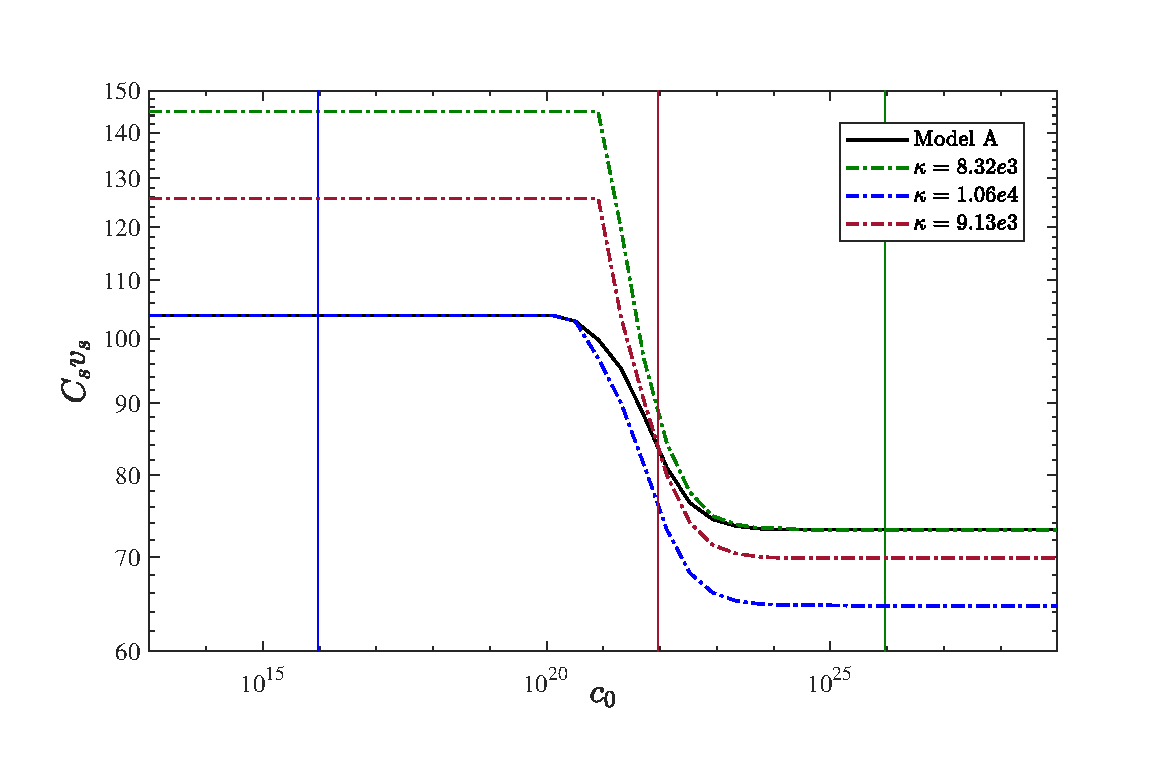
\includegraphics[scale=0.36]{images/freeswel1}
		\caption{$G^A_{eq}=5e3$}
	\end{subfigure}
	\begin{subfigure}{0.39\textwidth}
		\hspace{-8mm}
		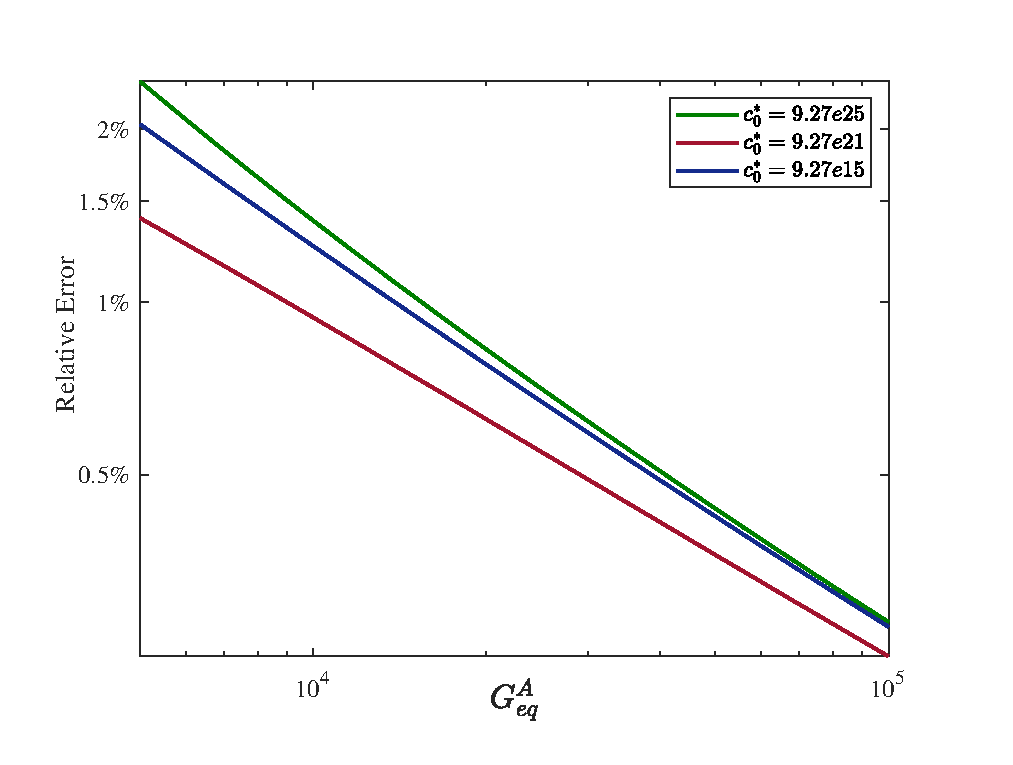
\includegraphics[scale=0.36]{images/freeswel2}
		\caption{}
	\end{subfigure}
	\vspace{3mm}
	\caption{Comparison of the prediction for the two models in a Free Swelling experiment. We consider as a reference Model A (ground truth). We fix the concentration $c^*_0$ of ions in the bath, we leave the matrix reach is steady state and we measure $C_s(c^*_0)$. Using Equations~(\ref{eqF})-(\ref{eqFb}) we have $\kappa(c^*_0)=G^A_{eq}((1+v_sC_s)^{2/3}-1)$. The same is repeated for three different salt concentration (each experiment correspond to a colour,see legend of Figure (b)). (a) 
		Comparison between Model A and Model B for the different estimated values $\kappa(c^*_0)$. (b) Relative error between the model as a function of the matrix stiffness $G_{eq}^A$. We note that the softer the matrix, the larger is the discrepancy between the two model. The choice of $c^*_0$ can also impact on the estimated error. Given the same mixing parameter $\chi$, the two models can not agree on the equilibrium behaviour for the two limits: $c_0$ small or $c_0$ large. Consequently the best choice would be choosing $c_0$ in the region of transition. Note that the shear modulus of the ECM is estimated to be of order $10^3-10^4$ \cite{Netti}.}
	\label{Exp1}
\end{figure}

If we consider instead the mixing parameter $\chi$ to be also unknown, then there is a set of parameter values for which the models predict the same equilibrium swelling fraction, see Figure \ref{freeA}. However, as illustrated in Figure \ref{freeB}, there are several order of magnitude of difference in the expected pressure inside the gel. Such discrepancy depend on the phase of the ECM. As discussed in \cite{}, polyelectrolytes can undergo a discontinuous phase transition between an highly swollen, i.e. $C_s>>1$, and a collapsed phase, i.e. $C_s\sim<1$. As shown in Figure \ref{freeC}, the state depends on the value of the mixing parameter $\chi$ and thus on the osmotic pressure $\Pi^n$ in the ECM. While the models agree in predicting the collapsed phase, i.e. small deformation, there is a great difference in the expected mixing properties in the case of large changes in the ECM volume. 

\begin{figure}[h]
	\begin{subfigure}{0.49\textwidth}
		\centering
		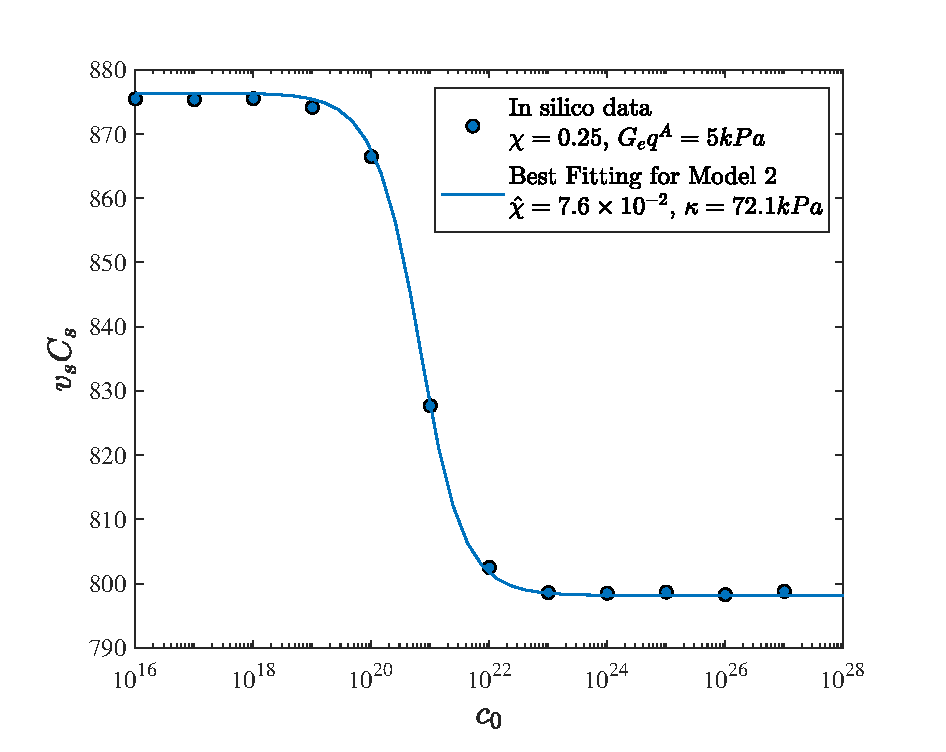
\includegraphics[scale=0.32]{images/chi2}
		\caption{}
		\label{freeA}
	\end{subfigure}	
	\begin{subfigure}{0.49\textwidth}
		\centering
		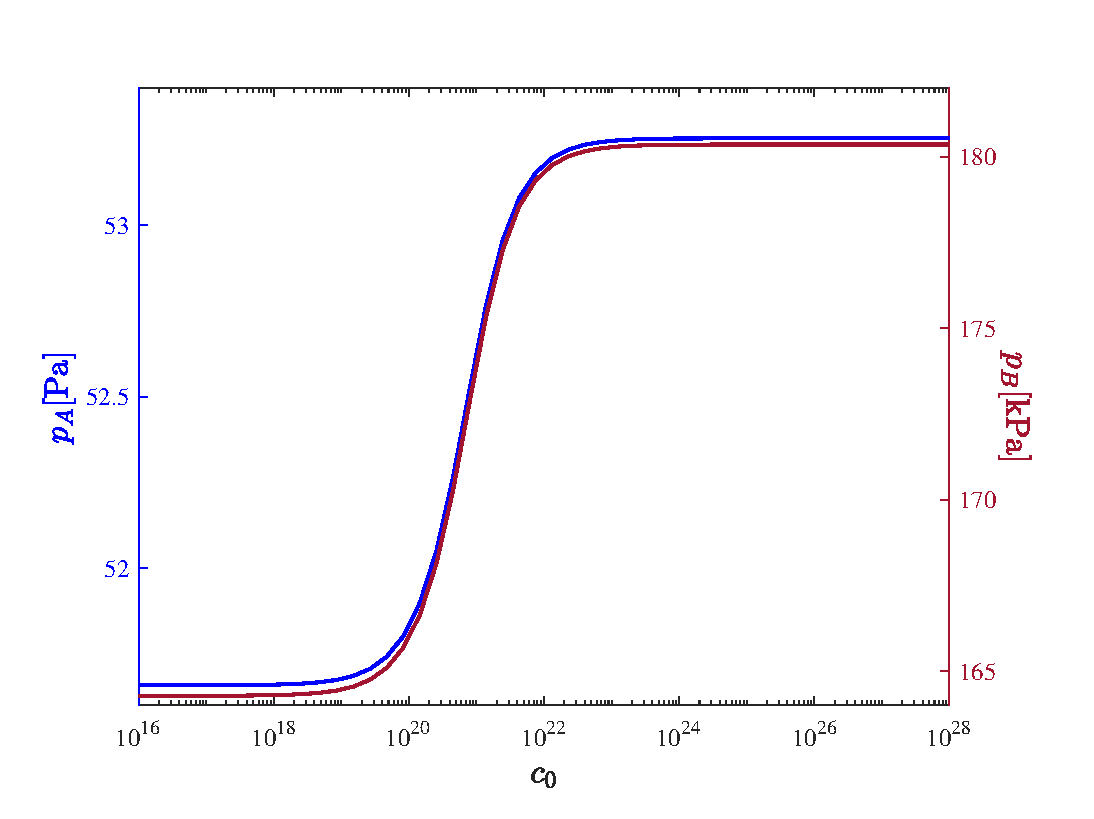
\includegraphics[scale=0.285]{images/chi3p}
		\caption{}
		\label{freeB}
	\end{subfigure}	
	
	\centering
	\begin{subfigure}{0.6\textwidth}
		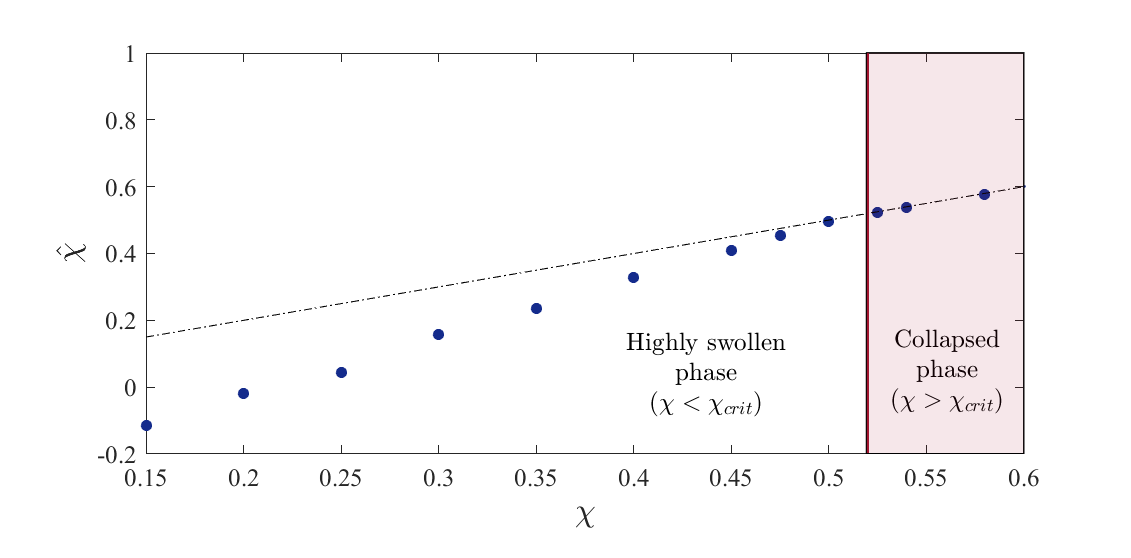
\includegraphics[scale=0.415]{images/chi1}
		\caption{}
		\label{freeC}
	\end{subfigure}
	\caption{Model Comparison 2: despite there is a set of parameters that would give rise to the same equilibrium behaviour this can drastically change the predicted mixing properties of the ECM. (a-b) Example of an \textit{in silico} experiment for $G^A_{eq}=5e2$: data are generated using model A and adding random noise. The fitting for model B is obtained using the non-linear least square method function in MATLAB, \texttt{fmincon}. (a) Predicted equilibrium concentration of water in the ECM; (b) Predicted mechanical pressure in the ECM from model A (blue) and model B (red). Despite capturing the same qualitative trend, the two differ of several order of magnitude. (c) Flory-Huggins parameter $\chi$ used in the \textit{in silico} experiment vs the one estimated fitting model B to the \textit{in silico} data $\hat{\chi}$; .}
	\label{figfree2}
\end{figure}

Based on our analysis, a simple unconstrained swelling experiment is informative only if, either $\chi$ is known or the pressure inside the ECM is known. However, when dealing with tissue, it is unlikely to be the case. Based on our current knowledge, there are no quantitative studies focusing on the value of $\chi$. Similarly, previous studies rely on mathematical models to estimate the pressure as experimentally measures can be challenging \cite{pressure,ecm1,ecm2}. 
\section{Confined Compression Test.}

\begin{figure}[h]
	\centering
	\def\svgwidth{0.89\linewidth}
	\input{latex/images/compression.pdf_tex}
	\vspace{2mm}
	\caption{Schematic representation of a compression test with a porous piston. A deformation is imposed in the $Z$ direction and the force necessary to maintain the deformation is recorded. }
\end{figure}

In this second example, we consider to perform on a swollen slice of ECM a compression test with the use of a porous platen,which allows the fluids to flow so to maintain the chemical equilibrium with the external bath \cite{Netti}. This allows to measure both the dynamical and equilibrium behaviour of the material by measuring the stress while imposing a known strain $\epsilon$. The corresponding deformation tensor is of the form:

\begin{equation}
\F=J_0^{1/3}\begin{bmatrix}
1 &0&0\\
0&1&0\\
0&0& \lambda_1
\end{bmatrix},
\label{F} 
\end{equation}
where $\lambda_1 = 1 - \epsilon$. 
\subsection{Model A}
As before, given the symmetries of the system, $\B_e$ is a diagonal matrix of the form:
\begin{equation}
\B_e=\begin{bmatrix}
b &0&0\\
0&b&0\\
0&0& b_1
\end{bmatrix}. 
\end{equation}
Again we are here interested in the equilibrium behaviour, for which Equations~(\ref{eqion}) still holds. Focusing on the contribution of spring B, studying the equilibriums of Equation~(\ref{Be}), we obtain that $b=b_1$. Since $\det \B_e= (\det \F)^2$, we conclude that:
\begin{equation}
b = J_0^{2/3}\lambda_1^{2/3}.
\end{equation}

Using the boundary condition, we can now compute the pressure and the equilibrium condition:
\begin{gather}
p = -\sigma + \frac{G^A_1}{J_0\lambda_1} (J^{2/3}_0\lambda_1^2-1)+\frac{G^A_2}{J_0\lambda_1} (J_0^{2/3} \lambda_1^{2/3}-1) \\
\begin{aligned}
\frac{\sigma v_s}{k_B T}=&\frac{J_0\lambda_1+\chi}{J_0^2\lambda^2_1}+\frac{G_1^Av_s}{k_BT} \frac{J_0^{2/3}\lambda^2_1-1}{J_0 \lambda_1}+\frac{G_2^Av_s}{k_BT} \frac{J_0^{2/3}\lambda^{2/3}_1-1}{J_0 \lambda_1}\\[1.5mm]
&+\ln \frac{J_0\lambda_1-1}{J_0\lambda_1} +2c_0v_s-\sqrt{\left(\frac{z_fC_fv_s}{J_0\lambda_1-1}\right)^2+4v_s^2c^2_0}\label{compA}
\end{aligned}
\end{gather}

\subsection{Models B.}
Based on Equation~(\ref{F}), we have that the tensors $\bar{\B}$ and $\bar{\B}_e$ are of the form:
\begin{equation}
\bar{\B}=\begin{bmatrix}
\lambda_1^{-2/3} &0&0\\
0&\lambda_1^{-2/3}&0\\
0&0& \lambda_1^{4/3}
\end{bmatrix}, \qquad
\bar{\B}_e=\begin{bmatrix}
\bar{b} &0&0\\
0&\bar{b}&0\\
0&0& \bar{b}_1
\end{bmatrix}
\end{equation}

As for the model A, at equilibrium we have that $\bar{b}=\bar{b}_1$. However, in this case, we have that $\det \bar{B}_e=1$ so that $\bar{b}=1$ so that the second spring does not contribute to the stress. Using the boundary condition, in the case of model $BA$ we obtain:
\begin{gather}
\displaystyle 
p_{BA} = -\sigma + \frac{G^A_{eq}}{J_0\lambda_1}(J_0^{2/3}\lambda_1^{2/3}-1)+\dfrac{2G^B_1}{3J_0\lambda_1^{5/3}} (\lambda_1^2-1) \\
\begin{aligned}
\frac{\sigma v_s}{k_B T}=&\dfrac{J_0\lambda_1+\chi}{J_0^2\lambda^2_1}+\frac{2G_1^Bv_s}{3k_BT} \dfrac{\lambda^2_1-1}{J_0 \lambda_1^{5/3}}+\frac{G^A_{eq}v_s}{k_BT}\frac{J_0^{2/3}\lambda_1^{2/3}-1}{J_0\lambda_1}\\[1.5mm]
& +\ln \frac{J_0\lambda_1-1}{J_0\lambda_1}+2c_0v_s-\sqrt{\left(\frac{z_fC_fv_s}{J_0\lambda_1-1}\right)^2+4v_s^2c^2_0}.\label{compAB}
\end{aligned}
\end{gather}

Unlike the case of unconstrained swelling, we now have that the model $A$ and $BA$ are substantially different, so that there is no choice of the parameter that would predict the same stress-strain behaviour. This highlights how, the choice of a particular decomposition of the deformation gradient $\F$ correspond to a modelling decision on the constitutive properties of the material under study.  
while for model $B$, the equilibrium conditions are:
\begin{gather}
\displaystyle 
p_B = -\sigma + \frac{\kappa}{J_0\lambda_1}+\dfrac{2G^B_1}{3J_0\lambda_1^{5/3}} (\lambda_1^2-1) \\
\begin{aligned}
\frac{\sigma v_s}{k_B T}=&\dfrac{J_0\lambda_1+\chi}{J_0^2\lambda^2_1}+\frac{2G_1^Bv_s}{3k_BT} \dfrac{\lambda^2_1-1}{J_0 \lambda_1^{5/3}}+\frac{\kappa v_s}{k_BT} \frac{1}{J_0 \lambda_1}+\ln \frac{J_0\lambda_1-1}{J_0\lambda_1}\\[1.5mm]
& +2c_0v_s-\sqrt{\left(\frac{z_fC_fv_s}{J_0\lambda_1-1}\right)^2+4v_s^2c^2_0}.
\end{aligned}
\end{gather}

\subsection{Model Comparison.}
We first focus on comparing the model $A$ and $AB$, assuming that the parameter $\chi$ is fixed and that $G^{AB}_{vol}=G^A_{eq}$, so that the equilibrium volume $J_0$ is the same for both models. If we now take the difference between Equations~(\ref{compA}) and (\ref{compAB}), we obtain that the difference in the compression stress $\delta \sigma= \sigma_{BA}-\sigma_{A}$ is:
\begin{equation}
\delta \sigma = \frac{2 G_1^{AB}}{3} \frac{\lambda_1^2-1}{J_0\lambda_1^{5/3}} - \frac{G_1^A}{J_0^{1/3}}(\lambda_1-\lambda_1^{-1/3}).\label{err}
\end{equation}
Looking at the above equation it appears clearly that there is no constant value of $G^{AB}_1$ for which the difference $\delta \sigma$ is identically zero. If we impose that for small deformation, i.e. $\lambda_1\rightarrow 1$, the two models agree at the second order:
\begin{equation}
\delta \sigma=0, \qquad \frac{\d \delta \sigma}{\d \lambda_1}=0 \quad\Rightarrow \quad G_1^{AB} = J_0^{2/3}G_1^A.
\end{equation}
Under such condition we can rewrite the Equation~(\ref{err}) as:
\begin{equation}
\delta \sigma(\lambda_1;G^A_1,J_0) = \frac{G_1^A}{J^{1/3}_0\lambda_1^{5/3}} \left(\frac{2}{3}\lambda^2_1-\frac{2}{3}-\lambda_1^{5/3}+\lambda_1^{4/3}\right), 
\end{equation}
which is unbounded for large deformation, i.e. $\lambda_1\Rightarrow0$.
%We here consider another standardd
\begin{figure}
	\hspace{-8mm}
	\begin{subfigure}{0.62\textwidth}
		\hspace{6mm}
		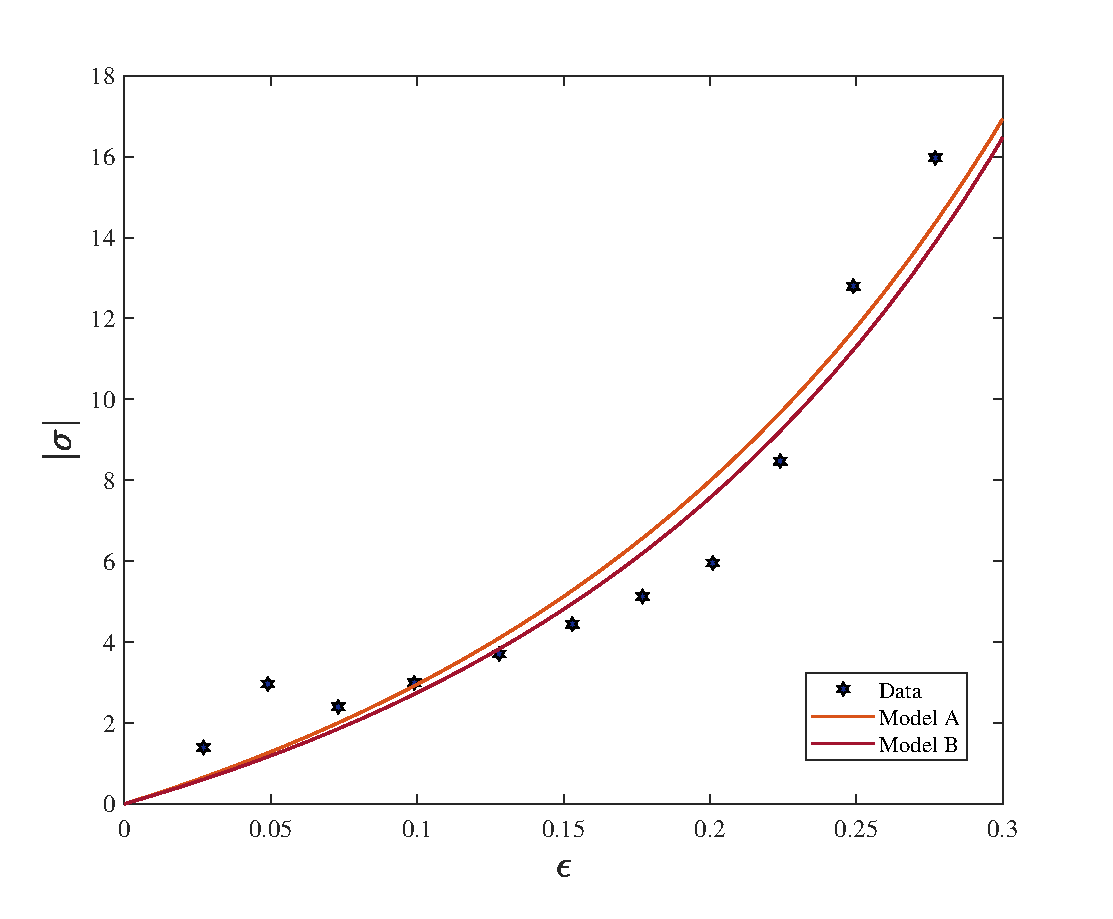
\includegraphics[scale=0.35]{images/compression.eps}
		\caption{Fitted Model}
		\label{fit}
	\end{subfigure}
	\begin{subtable}{0.375\textwidth}
			\begin{tabular}{c | c ||c| c }		
				\hline\addlinespace[2pt]
				 \multicolumn{2}{c||}{Model A} &  \multicolumn{2}{c}{Model B}\\[0.5mm]
				\hline\addlinespace[2pt]
				$\quad \chi\quad$ & $\quad0.498\quad$ &$\quad \chi\quad$&$\quad0.523\quad$\\[0.5mm]
				$G^A_1$ & 18.9 kPa&$\kappa$& 0.83 kPa\\[0.5mm]
				$G^A_2$ & 5.3 Pa&$G^B_1$& 55.1 kPa\\[0.5mm]
				$J_0$ & $20.7$&  $J_0$&$14.8$\\[0.5mm]
				\hline\addlinespace[2pt]
				\multicolumn{4}{c}{Model BA}\\[0.5mm]
				\hline\addlinespace[2pt]
				\multicolumn{2}{c|}{$\chi$} & \multicolumn{2}{c}{0.524}  \\
				\multicolumn{2}{c|}{$G_{vol}$} & \multicolumn{2}{c}{75 Pa}  \\
	            \multicolumn{2}{c|}{$G^{BA}_{1}$} & \multicolumn{2}{c}{55.1 kPa} \\
				\multicolumn{2}{c|}{$J_0$} & 	\multicolumn{2}{c}{ 14.8}\\
				\hline
			\end{tabular}
		\caption{Estimated Parameters}
		\label{param}
	\end{subtable}
\caption{Comparison of the two model in fitting real experimental data from \cite{Netti}.}		
\end{figure}

As shown in Figure \ref{fit}, both models are able to capture the qualitative behaviour of the data. However, as shown by the parameters in Table \ref{param}, there are quantitative differences. In particular, there are order of magnitude of difference in the estimated pressure $p$. If we look at its value for zero-strain, i.e. $\lambda_1=1$, we obtain: 
\begin{gather}
p_A = \frac{G^A_1+G^A_2}{J_0}(J_0^{2/3}-1) = \frac{24.2 \text{ kPa}}{20.7}(20.7^{2/3}-1) = 7.64 \text{ kPa},\\
p_{BA} = \frac{G_vol}{J_0}(J_0^{2/3}-1) = \frac{0.075 \text{ kPa}}{14.8}(14.8^{2/3}-1) = 25.5 \text{ Pa}\\
p_B = \frac{\kappa}{J_0} = \frac{0.83 \text{ kPa}}{14.8} = 56.08 \text{ Pa}
\end{gather}

When designing synthetic ECM, the tuning of the internal pressure cells in a culture are exposed to is of large importance. As mentioned in the introduction, cells are sensitive to pressure and their response can greatly change depending on this stimulus. Consequently, depending on the model chosen, the
